\subsection{Droplets and Molecules}
% ---------- Slide 1: 4He nanodroplets ----------
\begin{frame}{\texorpdfstring{$^4$He nanodroplets \& field coupling to linear molecules}{He-4 nanodroplets \& field coupling to linear molecules}}
\small
\begin{itemize}
  \item \textbf{$^4$He nanodroplets:} formed by supersonic expansion through a cryogenic nozzle; cool to
        \textbf{$\sim 0.4$ K} and are typically \textbf{superfluid}.
  \item \textbf{Size:} usually \textbf{$N \sim 10^{3}$--$10^{6}$ He atoms} $\Rightarrow$ radius \textbf{$10 - 100$ nm} 
        (source-condition dependent)\footcite{toennies2004superfluid}.
  \item \textbf{Molecule pickup:} droplets capture molecules in a pickup cell and rapidly \textbf{cool/thermalize} them.
  \item \textbf{E-field coupling (nonresonant):} alignment via anisotropic polarizability \footcite{MacPhailBartley2024SuperfluidHelium}
        \[
        U(t)\propto -\Delta\alpha\,E^2(t)\cos^2\theta,\qquad \Delta\alpha=\alpha_{\parallel}-\alpha_{\perp}.
        \]
  \item For $\Delta\alpha>0$ the molecule aligns with the instantaneous polarization axis; if that axis rotates
        (optical centrifuge), the molecule can be \textbf{captured and spun up} to high $J$.
\end{itemize}
\end{frame}

\begin{frame}{Spinning of NO dimers}
  \centering
  \begin{figure}
  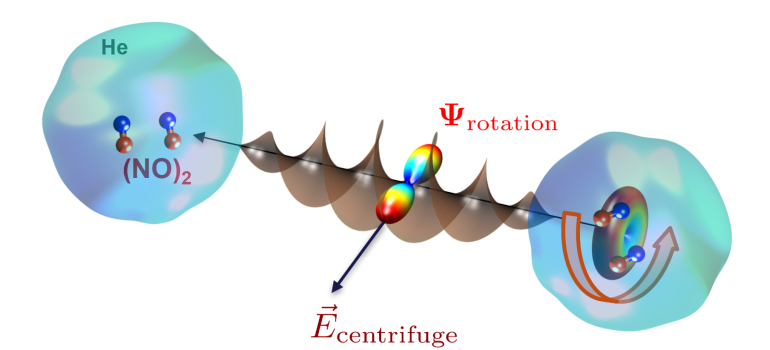
\includegraphics[width=.7\linewidth]{pic/droplets_molecules.png}
  \caption{Spinning of NO dimers in helium nanodroplets with optical centrifuge\footcite{milnerSite}}
  \end{figure}
\end{frame}